\section{碰 (40pts)}
瓦雷莎正在锻炼她的碰撞本领,她会去尝试冲撞一个静止的巨石。下面让我们来帮她分析一下情况,我们将他们抽象为两个质点,分别为\(m_1\)和\(m_2\),其中\(m_1\)为瓦雷莎,\(m_2\)为静止的巨石。瓦雷莎以初始动量\(p_0\)向右冲撞巨石,考虑相对论效应,已知光速为\(c\),则瓦雷莎初始能量为\(E_1 = \sqrt{p_0^2c^2 + m_1^2c^4}\)。如图\ref{peng1} 所示:
\begin{figure}[htbp]
	\centering
	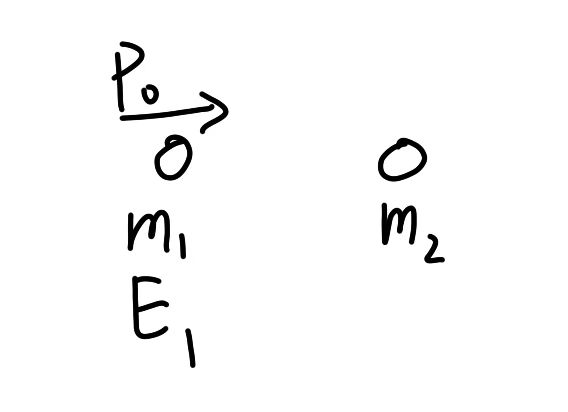
\includegraphics[width=0.3\textwidth]{peng1}
	\caption{碰撞示意图.}
	\label{peng1}
\end{figure}
\begin{enumerate}
	\item 我们先为这个分析打一个基础:已知空间中有\(n\)个质点,它们的动量分别为\(\vec{p}_1,\vec{p}_2,\cdots,\vec{p}_n\),能量分别为\(E_1,E_2,\cdots,E_n\),请你证明:存在一个参考系,它相对于当前参考系的速度为\(\vec{\beta}_c c\), 使得在这个参考系中,所有的质点的总动量为0,并求出\(\vec{\beta}_c\)的表达式。(12pts)
	\item 现在回来分析瓦雷莎的情况,请问什么情况下她会直接被巨石原路反弹?请给出条件,当不会反弹时,求出她的最大可能的偏离原来方向的角度。(28pts)
\end{enumerate}

\section*{Answer 3}
\begin{enumerate}
	\item 首先我们在实验系下找一个方向使得在这个方向上的总动量为0(这必然找得到,因为总动量是一个矢量,必然可以旋转坐标架做到这一点), 设这个方向为\(y\)轴,\(x\)轴为垂直于\(y\)轴的方向。现在令\(\beta_c\)方向沿着\(x\)轴,有:
	\begin{align*}
		\sum_{i=1}^{n} p_{i,y}' &= \sum_{i=1}^{n} p_{i,y}= 0 \\
		\sum_{i=1}^{n} p_{i,x}' &= \sum_{i=1}^{n} \gamma_c (p_{i,x} - \beta_c \frac{E_{i}}{c}) = 0 
	\end{align*}
	于是解的\(\beta_c\)为:
	\begin{align*}
		\beta_c &= \frac{\sum_{i=1}^{n} p_{i,x}c}{\sum_{i=1}^{n} E_{i}} 
	\end{align*}
	注意到所选轴的特殊性,有:
	\begin{align*}
		\vec{\beta}_c &= \frac{\sum_{i=1}^{n} \vec{p}_{i}c}{\sum_{i=1}^{n} E_{i}} 
	\end{align*}
	现在完全变成了矢量形式,与坐标架的选择无关了,证毕。
	\item 我们换到零动量系,也就是\(\vec{\beta}_c = \frac{\vec{p}_0 }{E_1 + m_2c^2}\),在这个系下,二者的动量大小相等方向相反,设大小为\(p'\), 有:
	\begin{align*}
		p' &= \gamma_c (p_0- \beta_c \frac{E_{1}}{c}) = \gamma_c \beta_c m_2 c \\
		E_1' &= \sqrt{p'^2c^2 + m_1^2c^4} = \gamma_c (E_1 -\beta_c p_0 c)\\
		E_2' &= \sqrt{p'^2c^2 + m_2^2c^4}
	\end{align*}
	在这个参考系下,碰撞前后的能量守恒与动量守恒会保证二者的动量大小相等方向相反,且大小仍为\(p'\)。(因为这里的解是唯一的,有两个方程。)唯一不同的只有方向,设偏向的角度为\(\theta\),将动量变换回去,得到:
	\begin{align*}
		p_{1,x} &= \gamma_c ( p' \cos \theta + \beta_c \frac{E_{1}'}{c}) \\
		p_{1,y} &= p' \sin \theta  
	\end{align*}
	因此,如果出现反弹的情况,必然有\(\theta = \pi\)时\(p_{1,x} < 0\), 也就是:
	\begin{align*}
		\frac{\beta_c E_1'}{p' c} < 1
	\end{align*}
	化简得:
	\begin{align*}
		\frac{E_1 m_2 + m_1^2 c^4}{E_1 m_2+ m_2^2 c^4} < 1 
	\end{align*}
	这也意味着:
	\begin{align*}
		m_1 < m_2
	\end{align*}
	所以只要瓦雷莎的质量大于巨石的质量,她就会不会被反弹。否则她会被反弹。当不会被反弹时:
	\begin{align*}
		tan\theta &= \frac{p_{1,y}}{p_{1,x}} = \frac{p' \sin \theta}{\gamma_c ( p' \cos \theta + \beta_c \frac{E_{1}'}{c})} 
	\end{align*}
	对上式求导令其为0,得到:
	\begin{align*}
		cos\theta = -\frac{p' c}{\beta_c E_1'} = -\frac{E_1 m_2 + m_2^2 c^4}{E_1 m_2+ m_1^2 c^4}
	\end{align*}
	可见也是只有在\(m_1 > m_2\)时,才有解。回代,得到:
	\begin{align*}
		tan\theta &= \frac{1}{\gamma_c \sqrt{(\frac{\beta_c E_1'}{p' c})^2-1}} 
	\end{align*}
	最终的结果为:
	\begin{align*}
		\theta &= \arctan \left(\frac{1}{\sqrt{1-(\frac{p_0}{E_1 + m_2c^2})^2}\sqrt{(\frac{E_1 m_2 + m_1^2 c^4}{E_1 m_2+ m_2^2 c^4})^2-1}} \right)
	\end{align*}

\end{enumerate}